\documentclass[11pt]{article}
\usepackage{certmachine}
\usepackage{graphicx}
%% generated by tools/paper-numbers/henon-entropy.js from certs/entropy-henon.json, certs/census-high-periods.json, the entropy battery (run live) and git — do not edit (git 054078d19462)
\newcommand{\RepoCommit}{054078d19462}
\newcommand{\HenonA}{1.4}
\newcommand{\HenonB}{0.3}
\newcommand{\NBoxes}{340}
\newcommand{\NEdges}{4{,}140}
\newcommand{\RecordHLBRaw}{0.3016800418811779}
\newcommand{\ComposedK}{11}
\newcommand{\ADouble}{1.3999999999999999112}
\newcommand{\BDouble}{0.29999999999999998890}
\newcommand{\AUlpLo}{1.3999999999999996891}
\newcommand{\AUlpHi}{1.4000000000000001332}
\newcommand{\BUlpLo}{0.29999999999999993339}
\newcommand{\BUlpHi}{0.30000000000000004441}
\newcommand{\UHalf}{0.0150}
\newcommand{\SHalf}{0.0048}
\newcommand{\HuntDelta}{0.03}
\newcommand{\UHalfFrac}{0.5}
\newcommand{\SHalfFrac}{0.16}
\newcommand{\AspectRatio}{3.13}
\newcommand{\XMin}{-1.26}
\newcommand{\XMax}{1.27}
\newcommand{\YMin}{-1.28}
\newcommand{\YMax}{1.27}
\newcommand{\DurMax}{6}
\newcommand{\EdgeRows}{1 & 101 & 101 & 2.4\% \\
2 & 254 & 355 & 6.1\% \\
3 & 442 & 797 & 10.7\% \\
4 & 751 & 1{,}548 & 18.1\% \\
5 & 1{,}099 & 2{,}647 & 26.5\% \\
6 & 1{,}493 & 4{,}140 & 36.1\% \\}
\newcommand{\EdgesKOne}{101}
\newcommand{\EdgesKTwo}{254}
\newcommand{\EdgesKThree}{442}
\newcommand{\EdgesKFour}{751}
\newcommand{\EdgesKFive}{1{,}099}
\newcommand{\EdgesKSix}{1{,}493}
\newcommand{\NPairs}{4{,}069}
\newcommand{\NMultiPairs}{51}
\newcommand{\NSelfLoops}{11}
\newcommand{\NNoOut}{19}
\newcommand{\NNoIn}{84}
\newcommand{\MaxOut}{41}
\newcommand{\MaxIn}{50}
\newcommand{\MeanOut}{12.2}
\newcommand{\UnionSCCs}{115}
\newcommand{\UnionSCCLargest}{226}
\newcommand{\UnionSCCSingletons}{114}
\newcommand{\CellBudget}{8{,}000}
\newcommand{\KMax}{40}
\newcommand{\MinWidth}{$1\times10^{-6}$}
\newcommand{\MaxM}{8}
\newcommand{\LimitExp}{49}
\newcommand{\PowerM}{8}
\newcommand{\CoreSize}{223}
\newcommand{\MKProduct}{88}
\newcommand{\MinRowSum}{338{,}518{,}196{,}978}
\newcommand{\MinRowSumRaw}{338518196978}
\newcommand{\BKOnes}{13{,}740}
\newcommand{\BKDensityPct}{11.9\%}
\newcommand{\ExactBound}{\tfrac{1}{88}\ln 338{,}518{,}196{,}978}
\newcommand{\HLB}{0.301680}
\newcommand{\HLBNine}{0.301680041}
\newcommand{\KShow}{20}
\newcommand{\KRows}{1 & 101 & 1 & -- & -- & 0 \\
2 & 254 & 4 & -- & -- & 0 \\
3 & 442 & 21 & -- & -- & 0 \\
4 & 764 & 118 & 8 & 87 & 0.139560 \\
5 & 1{,}218 & 156 & 8 & 624 & 0.160904 \\
6 & 2{,}070 & 193 & 8 & 8{,}706 & 0.188995 \\
7 & 2{,}651 & 197 & 8 & 477{,}649 & 0.233511 \\
8 & 4{,}261 & 204 & 8 & 7{,}989{,}313 & 0.248338 \\
9 & 6{,}412 & 216 & 8 & 239{,}701{,}315 & 0.267985 \\
10 & 9{,}689 & 217 & 8 & 3{,}681{,}671{,}706 & 0.275333 \\
11 & 13{,}740 & 223 & 8 & 338{,}518{,}196{,}978 & 0.301680 \\
12 & 19{,}191 & 225 & 8 & 1{,}337{,}304{,}416{,}700 & 0.290851 \\
13 & 25{,}542 & 226 & 8 & 30{,}220{,}717{,}975{,}943 & 0.298457 \\
14 & 32{,}893 & 226 & 8 & 157{,}232{,}454{,}255{,}130 & 0.291864 \\
15 & 40{,}667 & 226 & 7 & 35{,}320{,}068{,}333{,}815 & 0.297100 \\
16 & 48{,}158 & 226 & 7 & 76{,}084{,}728{,}649{,}545 & 0.285383 \\
17 & 55{,}461 & 226 & 7 & 516{,}229{,}991{,}371{,}881 & 0.284685 \\
18 & 61{,}195 & 226 & 6 & 4{,}212{,}458{,}986{,}282 & 0.269158 \\
19 & 65{,}937 & 226 & 6 & 5{,}216{,}938{,}231{,}247 & 0.256868 \\
20 & 69{,}426 & 226 & 6 & 16{,}451{,}969{,}591{,}183 & 0.253596 \\}
\newcommand{\FirstPositiveK}{4}
\newcommand{\BoundKTwelve}{0.290851}
\newcommand{\BoundKThirteen}{0.298457}
\newcommand{\BoundKTen}{0.275333}
\newcommand{\BoundKTwenty}{0.253596}
\newcommand{\CoreAtTwenty}{226}
\newcommand{\MRows}{8 & 12 & 0.3016 \\
16 & 25 & 0.3201 \\
24 & 38 & 0.3263 \\
32 & 51 & 0.3294 \\}
\newcommand{\BoundMThirtyTwo}{0.3294}
\newcommand{\FloatSp}{41.47}
\newcommand{\FloatBound}{0.3386}
\newcommand{\BatteryPass}{12}
\newcommand{\BatterySeconds}{24}
\newcommand{\LnTwoDigits}{0.693147180560}
\newcommand{\ControlBound}{0.693147181}
\newcommand{\ControlRelations}{4}
\newcommand{\BatteryReds}{5}
\newcommand{\RedRefusals}{3}
\newcommand{\RedByEdge}{3}
\newcommand{\RedBySlab}{0}
\newcommand{\CalH}{0.6}
\newcommand{\CalW}{0.17}
\newcommand{\CalX}{0.38}
\newcommand{\CalKappa}{0.0395}
\newcommand{\CalKappaDen}{12}
\newcommand{\CalA}{6}
\newcommand{\CalCells}{60{,}000}
\newcommand{\ControlDurOne}{4}
\newcommand{\ControlDurTwo}{0}
\newcommand{\ControlDurTwoSameSide}{4}
\newcommand{\IntervalRerunCertified}{4{,}140}
\newcommand{\IntervalRerunBound}{0.301680}
\newcommand{\IntervalRerunAll}{all}
\newcommand{\CensusRows}{13 & 418 & 0.4643 \\
14 & 648 & 0.4624 \\
15 & 1{,}082 & 0.4658 \\
16 & 1{,}696 & 0.4648 \\}
\newcommand{\CensusPMin}{13}
\newcommand{\CensusPMax}{16}
\newcommand{\CensusCount}{4}
\newcommand{\Ceiling}{0.4658}
\newcommand{\CeilingP}{15}
\newcommand{\CeilingN}{1{,}082}
\newcommand{\RatePMax}{0.4648}
\newcommand{\NPMax}{1{,}696}
\newcommand{\RatioPct}{65}
\newcommand{\RatioPctPMax}{65}
\newcommand{\GapNats}{0.1641}
\newcommand{\LnTwo}{0.6931}
\newcommand{\RatioLnTwoPct}{44}
\newcommand{\DefectOneBound}{0.61}
\newcommand{\DefectTrueApprox}{0.465}
\newcommand{\DefectTwoBound}{0.4812}
\newcommand{\LitValue}{0.4651}
\newcommand{\LnPhi}{0.4812}
\newcommand{\OrbitPoints}{400{,}000}
\newcommand{\NScales}{6}
\newcommand{\CandRho}{1.6}
\newcommand{\Transient}{1{,}000}
\newcommand{\RecordCommit}{a395c7b}
\newcommand{\RecordDate}{2026-08-25}
\newcommand{\SoundCommit}{f86248d}
\newcommand{\SoundDate}{2026-08-25}
\newcommand{\TaintedBound}{0.356403}
\newcommand{\TaintedBoxes}{228}
\newcommand{\TaintedEdges}{916}
\newcommand{\TaintedK}{4}
\newcommand{\TaintedShape}{uniform}
\newcommand{\RecordCommits}{2}
\newcommand{\FigEdgeOne}{6\to11}
\newcommand{\FigEdgeSix}{249\to5}
\newcommand{\FigEdgeSixK}{6}


\newcommand{\htop}{h_{\mathrm{top}}}
\newcommand{\sprad}{\operatorname{sp}}
\newcommand{\cover}[1]{\stackrel{#1}{\Longrightarrow}}

\title{A certified lower bound on the topological entropy of the classical H\'enon map:\\
covering relations composed to an exact integer spectral argument}
\author{\cmauthor}
\date{October 2026 --- draft v0.1 for review; every number interpolated from the record; machine-derived, not peer-reviewed; author list to be agreed}

\begin{document}
\maketitle

\begin{abstract}
For the H\'enon map $F(x,y)=(1-ax^2+by,\,x)$ at the classical parameters $a=\HenonA$, $b=\HenonB$ we prove
$\htop(F)\ge\ExactBound>\HLB$. The proof is a finite certificate: \NBoxes{} pairwise disjoint parallelograms
(h-sets) in the plane; \NEdges{} covering relations $N_i\Rightarrow N_j$ for the iterates $F^k$, $k=1,\dots,\DurMax$,
each decided as a finite set of strict inequalities in outward-rounded interval arithmetic with adaptive bisection;
the relations chained to the uniform iterate $F^{\ComposedK}$ as a binary relation on the h-sets; and an exact
integer bound on the spectral radius of that relation (the minimum row sum of its \PowerM{}th power on a
\CoreSize-vertex core is \MinRowSum). The one external theorem consumed is the covering-relation theorem of
Zgliczy\'nski and Gidea. The instrument is calibrated where the answer is known: at $a=\CalA$ the same code
certifies the full two-shift and returns $\ln 2$. The number is not claimed to improve any published bound. What
is offered is the decision grammar---every step either certifies or refuses, and no floating-point quantity decides
anything---and a public record that a \BatterySeconds-second battery re-proves in full, the certificate included.
Two defects of earlier versions of the verifier, each found because it produced a bound above the value the
literature reports for this map, are described together with what now guards them; the interim bound
\TaintedBound{} that one of them produced is named as tainted and withdrawn. The certified cycle counts of the same
laboratory put the growth rate of periodic points at \Ceiling, and the distance to it is stated as the open problem,
with the cheapest next step identified in the certificate itself.
\end{abstract}

\section{Introduction}

H\'enon introduced the map $F_{a,b}(x,y)=(1-ax^2+by,\,x)$ in 1976 as the simplest polynomial diffeomorphism of the
plane with a numerically observed strange attractor, at the parameters $a=1.4$, $b=0.3$ \cite{Henon76}. Fifty years
later the attractor at those parameters is still the standard test object of two-dimensional chaos, and the simplest
quantitative statement one can make about it, the topological entropy $\htop(F)$ of Adler, Konheim and McAndrew
\cite{AKM65}---the exponential growth rate of the number of orbit segments distinguishable at a fixed resolution---is
not known in closed form. The report that accompanies the record behind this paper quotes the value the literature
reports as approximately $\LitValue$ without naming its source; this draft repeats neither the value's provenance nor
any published rigorous bound, because none is pinned in the record from which every number here is interpolated.
Rigorous lower bounds for this map by covering relations exist in the literature and the author's understanding is
that they exceed the bound proved here; the comparison is the first item for reviewers (Section~\ref{sec:open}).

This paper proves one inequality, $\htop(F)\ge\ExactBound$, and its contribution is not the inequality. The method
is the covering-relations method of Zgliczy\'nski and Gidea \cite{ZG04}, the standard tool for computer-assisted
entropy bounds in low dimension. What is new here is the decision grammar and the public re-runnable record:
\begin{itemize}
\item every covering relation is decided as a finite set of strict interval inequalities, by adaptive bisection with
outward rounding, with refusal (budget exhausted, condition not resolved) as the only alternative to certification,
so that the verifier can refuse a true relation but cannot certify a false one;
\item relations of different durations are chained to one uniform iterate as a \emph{binary} relation on the
h-sets, so that no path multiplicity enters the count of itineraries;
\item the spectral radius is bounded from below in exact integer arithmetic, by a row-sum argument, never by a
floating-point eigenvalue;
\item the certificate is finite data (parallelogram matrices, an edge list) in a public file, and a battery
re-derives every relation, the disjointness of every pair and the bound in \BatterySeconds{} seconds at every build
of the repository and of this document.
\end{itemize}
The instrument was calibrated before any new number counted: at $a=\CalA$, deep in the horseshoe regime of Devaney
and Nitecki \cite{DN79}, it certifies the full two-shift and returns $\ln 2$ (Proposition~\ref{prop:cal}). Two
earlier versions of the verifier were wrong, and both were found the same way: they returned a bound above the
value the literature reports for this map, which is impossible for a lower bound that is sound. Section~\ref{sec:defects}
describes both defects as engineering of the verifier, names the interim number one of them produced, and states
what guards each today, including one guard that, as it runs, does not exercise what it was written to pin.

A word on vocabulary. \emph{Certified} is used in one sense only: a statement is certified when a finite set of
inequalities whose truth implies it has been evaluated in outward-rounded interval arithmetic, or in exact integer
arithmetic, and found to hold. Elsewhere we say \emph{decided} or \emph{proved}.

\section{Statement of results}

Throughout, $F=F_{a,b}$ with $a$ and $b$ the IEEE-754 doubles nearest $\HenonA$ and $\HenonB$,
\[
a=\ADouble\ldots,\qquad b=\BDouble\ldots,
\]
which are the objects the record is stated for (Remark~\ref{rem:params} extends this). $F$ is a diffeomorphism of
the plane since $b\ne0$. For a compact $F$-invariant set $\Lambda$ we write $\htop(F|_\Lambda)$ for the topological
entropy of the restriction; $\htop(F)$ denotes the supremum over compact invariant sets, which is the entropy of
the restriction to the nonwandering set when that set is compact, and every lower bound below is a bound on
$\htop(F|_\Lambda)$ for an explicit compact invariant $\Lambda$, so any convention monotone in compact invariant
subsets receives it.

\begin{theorem}\label{thm:main}
\[
\htop(F)\;\ge\;\ExactBound\;=\;\HLBNine\ldots\;>\;\HLB .
\]
\end{theorem}

The bound is an explicit real number: the $\PowerM$th root of the integer $\MinRowSum$ is a lower bound for the
spectral radius of a $\CoreSize\times\CoreSize$ zero--one matrix read off the certificate, and that matrix encodes
the uniform iterate $F^{\ComposedK}$; the decimal is the floating-point evaluation of $\ln(\MinRowSumRaw)/\MKProduct$,
truncated.

\begin{remark}[the parameters]\label{rem:params}
The record is stated for the doubles because the verifier takes its parameters as point intervals. The same
verifier accepts parameter intervals, and while this draft was prepared it was re-run with $a$ and $b$ replaced by
the one-ulp intervals
\[
\begin{aligned}
a&\in[\AUlpLo\ldots,\ \AUlpHi\ldots],\\
b&\in[\BUlpLo\ldots,\ \BUlpHi\ldots],
\end{aligned}
\]
which contain the rationals $7/5$ and $3/10$ (decided exactly, by cross-multiplication of the doubles' dyadic
expansions): \IntervalRerunAll{} \IntervalRerunCertified{} relations re-certified and the bound is unchanged
($\IntervalRerunBound$). Since nothing else in the proof depends on the parameters, Theorem~\ref{thm:main} holds
for every $(a,b)$ in that box, the rational parameters included. This re-run is performed by the macro builder of
this document at every build, but it is not yet part of the record, which is why the theorem is stated as it is.
\end{remark}

\begin{proposition}[calibration]\label{prop:cal}
Let $a=\CalA$, $b=\HenonB$, and let
\[
N_\pm=(\pm x_0,0)+\begin{pmatrix} w&\pm\kappa\\ 0&H\end{pmatrix}[-1,1]^2,\qquad
x_0=\CalX,\ w=\CalW,\ H=\CalH,\ \kappa=\frac{bH}{\CalKappaDen\,x_0}=\CalKappa\ldots
\]
The instrument certifies the four covering relations $N_\pm\cover{F}N_\pm$ and returns the bound
$\ln\sprad(J)=\ln2$ with $J$ the all-ones $2\times2$ matrix (printed $\LnTwoDigits$), i.e.\ $\htop(F_{6,0.3})\ge\ln 2$,
which is the entropy of the full two-shift that Devaney and Nitecki proved to be the nonwandering set of the map
for $a$ beyond an explicit threshold depending on $b$ \cite{DN79}.
\end{proposition}

The proposition is run, as a gate, before the certificate of Theorem~\ref{thm:main} is admitted to any page or
document of the repository (Section~\ref{sec:battery}).

\section{The method}\label{sec:method}

\subsection{h-sets and covering relations}

An \emph{h-set} is a parallelogram $N=c+A[-1,1]^2$ with $c\in\R^2$ and $A\in\R^{2\times2}$ invertible; the first
column of $A$ is the nominally expanding direction $u$, the second the nominally contracting direction $s$. In the
coordinates $t=A^{-1}(x-c)$ the set is the square $N_c=[-1,1]^2$, its \emph{exit set} is the pair of
$u$-edges $N_c^-=\{\pm1\}\times[-1,1]$ and its \emph{entry set} is the pair of lids $N_c^+=[-1,1]\times\{\pm1\}$.
This is the h-set of Zgliczy\'nski and Gidea \cite{ZG04} with one expanding and one contracting dimension, the
coordinate homeomorphism being affine.

Fix two h-sets $N_1,N_2$ and an integer $k\ge1$, and let
\[
g(t)=A_2^{-1}\bigl(F^k(c_1+A_1t)-c_2\bigr),\qquad t\in[-1,1]^2,
\]
be $F^k$ written from the coordinates of $N_1$ to those of $N_2$, $g=(g_u,g_s)$. The instrument certifies the
relation $N_1\cover{F^k}N_2$ when the following two conditions hold.
\begin{itemize}
\item[(A)] \emph{The slab condition.} $g([-1,1]^2)$ does not meet the two closed slabs $\{|u|\le1,\ |s|\ge1\}$:
every point of the image either has $|g_s|<1$ or has $|g_u|>1$.
\item[(B)] \emph{The edge condition.} $g_u<-1$ on one of the two $u$-edges $\{\pm1\}\times[-1,1]$ and $g_u>1$ on
the other.
\end{itemize}

\begin{lemma}\label{lem:cover}
If (A) and (B) hold then $N_1\cover{F^k}N_2$ is a covering relation in the sense of \cite{ZG04}.
\end{lemma}

\begin{proof}
The definition in \cite{ZG04} asks for a homotopy $h:[0,1]\times N_{1,c}\to\R^2$ with $h_0=g$ such that
$h_t(N_{1,c}^-)\cap N_{2,c}=\emptyset$ and $h_t(N_{1,c})\cap N_{2,c}^+=\emptyset$ for all $t$, and $h_1(u,s)=(\lambda u,0)$
with $|\lambda|>1$. Take, for $t\in[0,\tfrac12]$, $h_t=(g_u,(1-2t)g_s)$: on the exit set $|g_u|>1$ by (B), so its
image never meets $N_{2,c}$; a point of the image with $|g_u|\le1$ has $|g_s|<1$ by (A), hence $|(1-2t)g_s|<1$, so the
image never meets a lid. Then, for $t\in[\tfrac12,1]$, interpolate the $u$-coordinate linearly from $g_u$ to
$\lambda u$ with $\lambda=\pm2$, the sign chosen so that $\lambda u$ lies on the same side as $g_u$ on each
$u$-edge, and keep $s=0$: the $s$-coordinate is never $\pm1$, and on each $u$-edge both ends of the interpolation lie
strictly beyond $\pm1$ on the same side, hence so does every point between them. The end map is the linear model.
\end{proof}

The lids alone are not enough: an image that crosses from $u<-1$ to $u>1$ while passing above the target, with
$|g_u|\le1$ and $g_s>1$ on the way, satisfies (B) and avoids both lids, yet no point of $N_1$ lands in $N_2$ and the
homotopy of the lemma does not exist. This is the second defect of Section~\ref{sec:defects}.

\subsection{Deciding a relation}

Conditions (A) and (B) are decided by evaluating $g$ on sub-boxes of $[-1,1]^2$ in interval arithmetic and
bisecting what is not resolved. The arithmetic is the repository's single interval library: every IEEE-754 basic
operation returns the correctly rounded nearest double, so widening each computed bound outward by one unit in the
last place encloses the exact result; the library is tested against exact rational arithmetic on random operands,
and removing the widening turns that test red. The matrix $A_2^{-1}$ is itself enclosed in intervals from the exact
determinant formula, so the conditions are verified for the true parallelogram and not for a floating-point
approximation of it; a target whose determinant interval contains zero is refused.

For (A) a cell $[u_0,u_1]\times[s_0,s_1]$ is \emph{clear} when the enclosure of $g_s$ over it lies strictly inside
$(-1,1)$ or the enclosure of $g_u$ lies strictly outside $[-1,1]$; a cell that is not clear is bisected along its
longer side. For (B) the same is done on each $u$-edge, with the enclosure of $g_u$ required to lie strictly beyond
$-1$ or strictly beyond $+1$, the side recorded, and a change of side along one edge refused. The budget is
\CellBudget{} cells per condition and a minimum cell width of \MinWidth; exhausting either refuses the relation. For
$k>1$ the map is iterated $k$ times in intervals; the h-sets are small (half-lengths $\UHalf$ along $u$ and
$\SHalf$ along $s$, Section~\ref{sec:cert}) and the subdivision is adaptive, so the enclosures stay tight through
the composed nonlinearity. Nothing in this procedure can certify a relation for which (A) or (B) fails: every clear
cell is clear by a strict inequality on an enclosure of the true image.

\subsection{Disjointness}

Two parallelograms are proved disjoint by the separating-axis test: along each of the four edge normals, the
outward-rounded projections of the two sets are compared, and strict separation along any axis proves
disjointness. The test is conservative in the safe direction, since it can fail to separate sets that are disjoint
but never separates sets that intersect. Every pair of h-sets of a certificate is tested, and a pair not proved
disjoint refuses the whole certificate, because the itinerary argument below needs the h-sets to separate orbits.

\subsection{Chains, itineraries and entropy}

The one external theorem consumed is used as a black box, in the way Krawczyk's theorem \cite{Kra69} is consumed by
the existence certificates of the same laboratory.

\begin{theorem}[Zgliczy\'nski--Gidea \cite{ZG04}, as consumed]\label{thm:zg}
Let $(N_t)_{t\in\Z}$ be h-sets and $(f_t)_{t\in\Z}$ continuous maps with $N_t\cover{f_t}N_{t+1}$ for every $t$. Then
there are points $x_t\in N_t$, $t\in\Z$, with $f_t(x_t)=x_{t+1}$ for every $t$.
\end{theorem}

Let $N_0,\dots,N_{n-1}$ be pairwise disjoint h-sets and $\mathcal E$ a set of certified relations $(i,j,k)$, each
meaning $N_i\cover{F^k}N_j$. For an integer $K\ge1$ define the zero--one matrix
\[
B_K[i][j]=1\iff\exists\,(a_0,a_1,k_1),\dots,(a_{r-1},a_r,k_r)\in\mathcal E:\ a_0=i,\ a_r=j,\ k_1+\dots+k_r=K .
\]
$B_K$ is computed by the recurrence $B_K=\bigvee_{k}A_k\cdot B_{K-k}$ over the duration matrices $A_k$ of
$\mathcal E$, with $B_0=I$, every product read as a boolean product. Nothing is claimed about $F^K$ covering
$N_j$ from $N_i$ when $B_K[i][j]=1$; the entry records the existence of a chain, and the uniform iterate enters only
through the times at which itineraries are read.

\begin{lemma}\label{lem:ent}
With the notation above, $\htop(F)\ge\frac1K\ln\sprad(B_K)$.
\end{lemma}

\begin{proof}
Let $\Sigma\subseteq\{0,\dots,n-1\}^\Z$ be the set of sequences $(i_m)$ with $B_K[i_m][i_{m+1}]=1$ for all $m$, a
vertex shift of finite type with $\htop(\sigma|_\Sigma)=\ln\sprad(B_K)$ \cite[Chapter 4]{LM95}. Let
$\Lambda=\{x:F^{mK}(x)\in\bigcup_iN_i\text{ for all }m\in\Z\}$: it is compact, since $F$ is a homeomorphism and the
union is compact, and $F^K$-invariant. Because the $N_i$ are compact and pairwise disjoint, the index of the h-set
containing a point is locally constant on their union, so $\pi:\Lambda\to\{0,\dots,n-1\}^\Z$,
$\pi(x)_m=$ the index of the h-set containing $F^{mK}(x)$, is well defined and continuous, and $\pi\circ F^K=\sigma\circ\pi$.
Given $(i_m)\in\Sigma$, choose for each $m$ a chain of total duration $K$ from $i_m$ to $i_{m+1}$ and concatenate the
chains into a bi-infinite sequence of certified relations; Theorem~\ref{thm:zg} gives points following it, and since
each $F^k$ is injective they are the orbit of one point $x$, which visits $N_{i_m}$ at time $mK$ for every $m$. Thus
$x\in\Lambda$ and $\pi(x)=(i_m)$, so $\Sigma\subseteq\pi(\Lambda)$. The image $\pi(\Lambda)$ is compact and
$\sigma$-invariant, and a factor has at most the entropy of the system, so
$\htop(F^K|_\Lambda)\ge\htop(\sigma|_{\pi(\Lambda)})\ge\htop(\sigma|_\Sigma)=\ln\sprad(B_K)$, the middle
inequality by monotonicity in closed invariant subsets. Finally $\htop(F^K|_\Lambda)=K\,\htop(F|_\Lambda)$
\cite[Chapter 7]{Wal82}, and $\Lambda$ is $F$-invariant after replacing it by $\bigcup_{r<K}F^r(\Lambda)$, which
does not change the entropy of $F^K$ on it.
\end{proof}

The lemma is where the first defect of Section~\ref{sec:defects} lived: with mixed durations, two chains that cut
the same span $K$ differently (a duration-two relation, or two duration-one relations through an intermediate
h-set) can be realised by one and the same orbit, because a duration-two relation constrains nothing at its
intermediate time. Counting chains overcounts orbits; $B_K$ is binary precisely so that an itinerary is a sequence of
h-sets read at the uniform times $mK$, where disjointness separates orbits.

\subsection{The exact spectral bound}

\begin{lemma}\label{lem:spec}
Let $B$ be a square matrix with nonnegative integer entries, $S$ a set of indices and $B_S$ the principal submatrix
on $S$. If every row sum of $B_S^{\,m}$ is at least $c>0$, then $\sprad(B)\ge\sprad(B_S)\ge c^{1/m}$.
\end{lemma}

\begin{proof}
The spectral radius of a nonnegative matrix dominates that of each principal submatrix \cite[Chapter 8]{HJ85}. If
$B_S^{\,m}\mathbf 1\ge c\,\mathbf 1$ entrywise then $B_S^{\,mr}\mathbf 1\ge c^r\mathbf 1$ for every $r$, so the row-sum
norm of $B_S^{\,mr}$ is at least $c^r$ and $\sprad(B_S)^m=\sprad(B_S^{\,m})\ge c$ by the spectral radius formula.
\end{proof}

The instrument trims $B_K$ to the set $S$ of indices that keep a positive row sum and a positive column sum within
$S$ (iterated to a fixed point), forms the powers $B_S^{\,m}$ for $m\le\MaxM$ in integer arithmetic guarded against
exceeding $2^{\LimitExp}$ (so that every partial sum stays below $2^{53}$ and the double arithmetic is exact), and keeps
the best value of $\ln(\min_i(B_S^{\,m}\mathbf 1)_i)/m$ over $m$ and over $K\le\KMax$; the macro builder of this document
recomputes the chosen row sum independently in arbitrary-precision integers. The bound is therefore
$\frac1K\ln c^{1/m}$ for an explicit integer $c$: a logarithm of an integer, never an eigenvalue.

\subsection{The proposer}

The h-sets and the candidate relations are proposed by a floating-point layer that is believed about nothing. A
float orbit of \OrbitPoints{} points after a transient of \Transient{} samples the numerically observed attractor;
binning at cell size $\delta$ keeps about one centre per occupied cell; each h-set takes its $u$-direction from the
principal axis of the orbit points in its cell and its $s$-direction from a few backward iterations of the
Jacobian, the standard float proposal for the stable direction; a greedy pass keeps a subset proved pairwise
disjoint by the certified test. A relation $(i,j,k)$ is nominated when the float image under $F^k$ of the
$u$-segment of $N_i$ passes within $\CandRho\,\delta$ of the centre of $N_j$. The hunt tries \NScales{} scales and
keeps the best certified bound. The record keeps only what survived certification; the number of nominated
relations is not recorded.

\subsection{Proof of Theorem~\ref{thm:main}}

The record \texttt{certs/entropy-henon.json} holds \NBoxes{} h-sets with half-lengths $\UHalf$ along $u$ and
$\SHalf$ along $s$ (the hunt's scale $\delta=\HuntDelta$ times $\UHalfFrac$ and $\SHalfFrac$), and \NEdges{} relations
$(i,j,k)$ with $k\le\DurMax$. The battery re-derives, from the record alone: that all $\binom{\NBoxes}{2}$ pairs of
h-sets are disjoint by the certified test; that each of the \NEdges{} relations satisfies (A) and (B) under the
procedure of Section~\ref{sec:method} within budget; and, by the recurrence, that $B_{\ComposedK}$ has a core $S$
of \CoreSize{} indices on which $B_S^{\,\PowerM}$ has minimum row sum $\MinRowSum$. Lemmas~\ref{lem:cover},
\ref{lem:ent} and~\ref{lem:spec} give
$\htop(F)\ge\frac1{\ComposedK}\ln\sprad(B_{\ComposedK})\ge\frac{1}{\MKProduct}\ln\MinRowSum$. \qed

\section{The certificate in numbers}\label{sec:cert}

Table~\ref{tab:dur} lists the relations by duration. Longer durations dominate: the single-step expansion of the
map at these parameters averages well below the factor that stretches a cell across a neighbour, so most of the
stretching the certificate uses is accumulated over several iterates, with the adaptive subdivision absorbing the
composed nonlinearity. The relations connect \NPairs{} distinct ordered pairs of h-sets; \NMultiPairs{} pairs carry
more than one duration and \NSelfLoops{} relations are loops $N_i\cover{F^k}N_i$. The mean out-degree is \MeanOut,
the largest out-degree \MaxOut{} and the largest in-degree \MaxIn; \NNoOut{} h-sets have no outgoing relation and
\NNoIn{} no incoming one, and the union graph over all durations has \UnionSCCs{} strongly connected components, one
of \UnionSCCLargest{} vertices and the rest singletons. Figure~\ref{fig:hsets} draws the h-sets; Figure~\ref{fig:rel}
draws one relation of each extreme duration in the target's coordinates, and the calibration pair.

\begin{table}[h]\centering\small
\begin{tabular}{rrrr}\toprule
duration $k$ & relations $N_i\cover{F^k}N_j$ & cumulative & share\\\midrule
\EdgeRows
\bottomrule\end{tabular}
\caption{The \NEdges{} certified covering relations by duration.}\label{tab:dur}
\end{table}

\begin{figure}[t]\centering
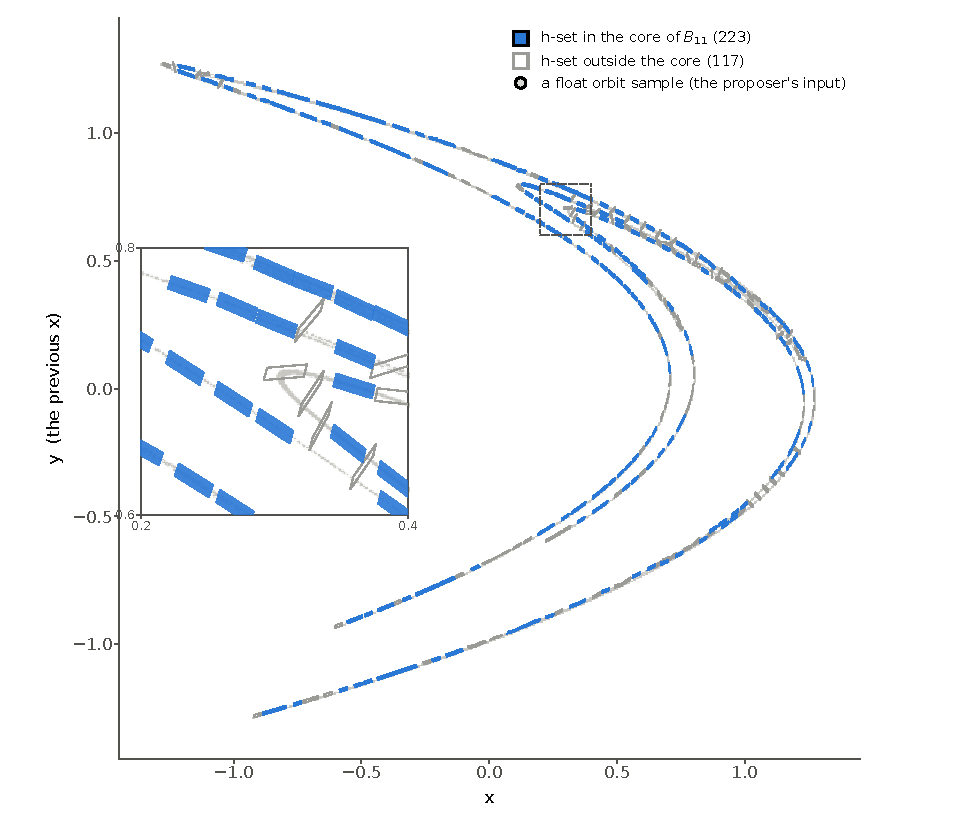
\includegraphics[width=0.68\linewidth]{fig/henon-entropy-hsets.pdf}
\caption{The \NBoxes{} h-sets of the record, drawn from the certificate: filled, the \CoreSize{} in the core of
$B_{\ComposedK}$; outlined, the rest; each a parallelogram with half-lengths $\UHalf$ and $\SHalf$. The grey points
are a float orbit sample, the proposer's input, for orientation only. The inset is the $0.2$-wide window holding
the most core h-sets, at scale.}\label{fig:hsets}
\end{figure}

\begin{figure}[t]\centering
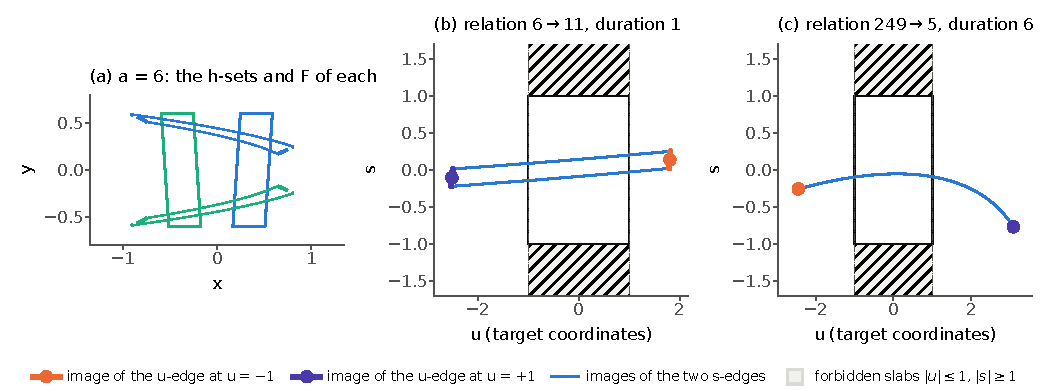
\includegraphics[width=0.96\linewidth]{fig/henon-entropy-relations.pdf}
\caption{(a) The calibration of Proposition~\ref{prop:cal} at $a=\CalA$: the two h-sets and the images of their
boundaries under $F$; each image is a long thin strip that crosses both h-sets, which is the full horseshoe.
(b)~The first relation of the record, $\FigEdgeOne$ at duration~1, and (c) the duration-$\FigEdgeSixK$ relation
whose image is shortest, $\FigEdgeSix$, both in the target's coordinates: the target is the unit square, the
hatched regions are the slabs that condition (A) forbids, the heavy marks are the images of the two $u$-edges,
which condition (B) places strictly beyond $u=\pm1$ on opposite sides. The curves are float images for the eye;
the certificate is the interval evaluation of Section~\ref{sec:method}.}\label{fig:rel}
\end{figure}

Table~\ref{tab:K} shows the composed bound for every uniform iterate $K\le\KShow$: the number of ordered pairs
with a duration-exactly-$K$ chain, the size of the core $S$, the power $m$ at which the row-sum bound is best and
that row sum. The first positive bound appears at $K=\FirstPositiveK$; the bound rises to its maximum at
$K=\ComposedK$ and falls afterwards (\BoundKTwelve{} at $K=12$, \BoundKThirteen{} at 13, \BoundKTwenty{} at
\KShow), because $B_K$ saturates towards the all-ones matrix on its \CoreAtTwenty-vertex core while the divisor $K$
keeps growing; the instrument's search to $K=\KMax$ finds nothing above $K=\ComposedK$. The entry at
$K=\ComposedK$ is Theorem~\ref{thm:main}.

\begin{table}[h]\centering\small
\begin{tabular}{rrrrrr}\toprule
$K$ & pairs with a chain & core $|S|$ & $m$ & $\min_i (B_S^{\,m}\mathbf 1)_i$ & $\frac{1}{mK}\ln(\cdot)$\\\midrule
\KRows
\bottomrule\end{tabular}
\caption{The composed bound for every uniform iterate $K\le\KShow$, recomputed from the recorded relations. A dash
means that no power gives a row sum above one there, so the bound is zero.}\label{tab:K}
\end{table}

\paragraph{The ceiling.} The same laboratory's census instrument counts the period-$p$ points of the map exactly:
it confines the plane by a certified a priori bound, excludes boxes by interval iteration, resolves the survivors
by Krawczyk's operator into boxes holding exactly one periodic point each, and decides identity and minimal period
by certificates rather than tolerances; a refusal is possible, a wrong count is not. Its one-off records for
$p=\CensusPMin,\dots,\CensusPMax$ at the classical parameters are in Table~\ref{tab:census}. For a $C^{1+\alpha}$ surface
diffeomorphism the exponential growth rate of periodic points dominates the entropy asymptotically \cite{Kat80}, which is
why the report calls the largest certified rate, $\Ceiling$ at $p=\CeilingP$, the \emph{ceiling}: it is where the counts
point, and it sits beside the value the report attributes to the literature, $\LitValue$. Finitely many counts bound
nothing, in either direction. The rate at the largest certified period, $p=\CensusPMax$ with $\NPMax$ points, is
$\RatePMax$, the figure the laboratory's handoff notes quote. Theorem~\ref{thm:main} is \RatioPct\% of the ceiling and
\RatioLnTwoPct\% of $\ln 2$; the gap of $\GapNats$ nats is the open problem, drawn to scale on the report page.

\begin{table}[h]\centering\small
\begin{tabular}{rrr}\toprule
period $p$ & points of period $p$, exact & $\ln(N_p)/p$\\\midrule
\CensusRows
\bottomrule\end{tabular}
\caption{The certified cycle counts of the census record \texttt{certs/census-high-periods.json} (points of period
$p$, i.e.\ fixed points of $F^p$, plane exhausted).}\label{tab:census}
\end{table}

\section{Calibration and controls}\label{sec:battery}

The gate of the instrument, \texttt{instruments/entropy/battery.js}, runs \BatteryPass{} checks in about
\BatterySeconds{} seconds and refuses the build on any failure; the macro builder of this document runs it live, so
the counts in this section are those of the run that produced the PDF.
\begin{enumerate}
\item The calibration of Proposition~\ref{prop:cal}: the two h-sets at $a=\CalA$, all four relations certified for
$F$ itself with a budget of \CalCells{} cells, the bound equal to $\ln2$ to twelve digits.
\item Three refusal controls: a target the image never reaches, a target too wide for the stretch, and a target
rotated so that the image crosses its lids, must each be refused. All three are refused, and the battery prints the
verifier's reason: in the run behind this document all \RedRefusals{} were decided by the edge condition (B)
(\RedByEdge{} of \RedRefusals), none by the slab condition (A). This is a finding about the gate: condition (A), the one
whose earlier form was the second defect of Section~\ref{sec:defects}, is not exercised by any refusal control
today.
\item Two h-sets that overlap must refuse the whole graph; they do.
\item The spectral routine on hand matrices: the full two-graph gives exactly $\ln2$ at every power, a single
two-cycle gives exactly $0$, an acyclic graph gives $0$.
\item A semantic control for the first defect: the calibration h-sets offered both duration-one and duration-two
candidates must still bound by $\ln2$. The control passes (\ControlBound, \ControlRelations{} relations). The
macro builder of this document re-runs its eight candidates one by one: the \ControlDurOne{} duration-one
relations certify and all \ControlDurTwoSameSide{} duration-two candidates are refused, because under $F^2$ the
images of both exit edges of either h-set land on the same side of the target, which is the fold of the horseshoe.
The refusals are expected; the consequence is that the composition of durations is not exercised by this control
as it runs, and the first defect is excluded by the construction of $B_K$ rather than by a control that would fire
on its return. A control in which duration-two relations do certify is listed in Section~\ref{sec:open}.
\item The certificate itself: the \NBoxes{} h-sets re-proved pairwise disjoint, every one of the \NEdges{}
relations re-derived, and the bound recomputed and found no lower than the recorded $\HLB$.
\end{enumerate}

\section{Two defects found by impossible numbers}\label{sec:defects}

Both defects were in the verifier, not in the method, and both were found by the same screen: a lower bound that
lands above the value the literature reports for this map is a bug until proved otherwise. Neither was found by
reading code. We state them as engineering of the verifier.

\paragraph{Mixed durations counted as itineraries.} The first version composed durations by counting: the number of
chains of total duration $K$ from $i$ to $j$ was taken as the $(i,j)$ entry of a matrix whose spectral radius was then
bounded. As explained after Lemma~\ref{lem:ent}, two chains that cut the same span differently can be realised by one
orbit, so the count overstates the number of distinguishable orbits. On the classical map the count returned
$h\ge\DefectOneBound$ against a literature value near $\DefectTrueApprox$. The fix is the binary $B_K$ of
Lemma~\ref{lem:ent}; the guard is the semantic control of Section~\ref{sec:battery}, with the caveat recorded there.

\paragraph{The lids-only image condition.} The first committed version of the verifier required the image to avoid
only the two lid segments $\{|u|\le1,\ s=\pm1\}$, the literal entry set, rather than the slabs of condition (A). An
image that arches over the target satisfies that condition and (B) without meeting the target, and Lemma~\ref{lem:cover}
has no proof for it. It was found because a two-h-set graph under $F$ at the classical parameters certified with a
bound converging to $\ln\varphi=\DefectTwoBound$ ($\varphi$ the golden ratio), above $\LitValue$. The fix is the slab
condition. The record committed under the lids-only condition, \texttt{\RecordCommit} of \RecordDate, stated
\[
\htop(F)\ \ge\ \TaintedBound\qquad\text{(tainted; withdrawn)}
\]
from \TaintedEdges{} relations of the single uniform iterate $F^{\TaintedK}$ over \TaintedBoxes{} h-sets; it was replaced
the same day by \texttt{\SoundCommit}, which carries the certificate of Theorem~\ref{thm:main}, and the record has
\RecordCommits{} versions in its history. The interim number is named here so that it cannot be quoted as a result: its
certificate does not establish it, and nothing here decides whether the inequality itself is true.

The lesson the laboratory drew is procedural and is now standing practice: calibrate where the answer is known
before any new number counts, and treat a bound above a credible reference value as a detector. The two reference
values used here, the literature's $\LitValue$ and the certified ceiling $\Ceiling$, are not inputs to any proof; they
are the alarms.

\section{What is not claimed}

\begin{itemize}
\item \emph{The value.} Nothing here estimates $\htop(F)$; Theorem~\ref{thm:main} is a lower bound and the ceiling is a
count.
\item \emph{An upper bound.} No statement here bounds the entropy from above. The census counts are consistent
with the reported literature value but bound nothing at finite period.
\item \emph{Priority or improvement.} The author's understanding is that published rigorous lower bounds for this map
exceed $\HLB$. They are not cited because none is pinned in the record; the claim of this paper is the grammar and
the record, not the number.
\item \emph{The rational parameters, as recorded.} The record is for the doubles; Remark~\ref{rem:params} reports a
re-run with one-ulp parameter intervals, performed at every build of this document and not yet part of the record.
\item \emph{The attractor.} The h-sets sit near a numerically observed attractor, but the invariant set $\Lambda$ of
Lemma~\ref{lem:ent} lives inside the h-sets and nothing is claimed about any other invariant set, about hyperbolicity,
or about the semi-conjugacy being a conjugacy.
\item \emph{Optimality of the certificate.} The proposer used one cell size and one pair of half-lengths for every
h-set; the certificate is one point in a large design space.
\end{itemize}

\section{The gap and the next step}\label{sec:open}

The gap of $\GapNats$ nats to the ceiling has three parts, and the certificate itself says which is cheapest.

\paragraph{The spectral step.} The record bounds $\sprad(B_{\ComposedK})$ by a row sum at power $m=\PowerM$. The
same matrix supports more: Table~\ref{tab:m} continues the exact integer row sums of $B_S^{\,m}$ to $m=32$ by vector
iteration (the macro builder of this document computes them; they are not in the record), and a floating-point
power iteration on the same core, an indication and not a certificate, puts $\ln\sprad(B_S)/\ComposedK$ near
$\FloatBound$. A certified Collatz--Wielandt inequality, $\sprad(B_S)\ge\min_i(B_Sv)_i/v_i$ for one explicit positive
rational vector $v$ evaluated exactly, would recover most of that from the recorded relations alone, with no new
interval work. This is the recommended first step.

\begin{table}[h]\centering\small
\begin{tabular}{rrr}\toprule
power $m$ & decimal digits of $\min_i(B_S^{\,m}\mathbf 1)_i$ & $\frac{1}{m\cdot\ComposedK}\ln(\cdot)$\\\midrule
\MRows
\bottomrule\end{tabular}
\caption{The row-sum bound on the recorded core of $B_{\ComposedK}$ continued past the recorded power, in exact
integers (truncated logarithms). The row $m=\PowerM$ is Theorem~\ref{thm:main}; the rest is not in the record.}\label{tab:m}
\end{table}

\paragraph{The h-sets.} All \NBoxes{} share one shape. Sizing each h-set to the local expansion, admitting longer
durations (the share of certified relations grows with $k$ in Table~\ref{tab:dur}), and densifying the core are the
recorded next steps of the report; each is new interval work and each is re-proved by the same battery.

\paragraph{The record.} Two bookkeeping items follow from this draft: the parameter intervals of
Remark~\ref{rem:params} should enter the record so that the theorem can be stated for $7/5$ and $3/10$; and two
controls should be added to the battery, one in which duration-two relations do certify so that the composition of
durations is exercised, and one with an image that arches over its target so that condition (A) is the condition
that refuses.

\paragraph{The comparison.} The published rigorous bounds for this map, and the provenance of the value
$\LitValue$ the report quotes, should be pinned in the corpus and cited; this draft does neither.

\cmrepro{The record is \path{certs/entropy-henon.json} (\RecordCommits{} versions; the one in force since
\texttt{\SoundCommit}, \SoundDate); the ceiling is \path{certs/census-high-periods.json}; the verifier is
\path{instruments/entropy/covering.js} and its gate \path{instruments/entropy/battery.js}
(\texttt{node} \path{instruments/entropy/battery.js}: about \BatterySeconds{} seconds, \BatteryPass{} checks, re-deriving
every relation of the certificate); the proposer is \path{tools/hunt-entropy.js} (re-running it rewrites the record);
the report page is \path{reports/entropy.html}, built by \path{tools/build-report-entropy.js}, which re-verifies the
certificate and re-runs the calibration before writing a byte; it is served at
\url{https://carlostoledo.co/reports/entropy.html}, with the record at
\url{https://carlostoledo.co/certs/entropy-henon.json}.
The macros of this document are written by \texttt{node} \path{tools/paper-numbers/henon-entropy.js}, which reads
the records, runs the battery, recomputes the composed bound through the instrument and through its own
implementation of the recurrence, confirms the row sum in arbitrary-precision integers, performs the one-ulp re-run
of Remark~\ref{rem:params}, and refuses when a record no longer supports a sentence; the figures are drawn by
\path{tools/paper-numbers/henon-entropy-figs.py}; the document is compiled by
\texttt{node} \path{tools/build-paper-tex.js} \texttt{henon-entropy}. Repository:
\url{https://github.com/carlostoledo1891/cert-machine}, concept DOI
\href{https://doi.org/10.5281/zenodo.22800699}{10.5281/zenodo.22800699}; this build is at commit
\texttt{\RepoCommit}.}

\begin{thebibliography}{9}\footnotesize
\bibitem{Henon76} M.~H\'enon, A two-dimensional mapping with a strange attractor, Comm.\ Math.\ Phys.\ 50 (1976),
69--77.
\bibitem{AKM65} R.~L.~Adler, A.~G.~Konheim, M.~H.~McAndrew, Topological entropy, Trans.\ Amer.\ Math.\ Soc.\ 114
(1965), 309--319.
\bibitem{ZG04} P.~Zgliczy\'nski, M.~Gidea, Covering relations for multidimensional dynamical systems, J.\ Differential
Equations 202 (2004), 32--58. The statement consumed is Theorem~\ref{thm:zg}, as recorded in the instrument's header
and the report page.
\bibitem{DN79} R.~Devaney, Z.~Nitecki, Shift automorphisms in the H\'enon mapping, Comm.\ Math.\ Phys.\ 67 (1979),
137--146.
\bibitem{Kra69} R.~Krawczyk, Newton-Algorithmen zur Bestimmung von Nullstellen mit Fehlerschranken, Computing 4
(1969), 187--201.
\bibitem{LM95} D.~Lind, B.~Marcus, An Introduction to Symbolic Dynamics and Coding, Cambridge University Press, 1995.
\bibitem{Wal82} P.~Walters, An Introduction to Ergodic Theory, Graduate Texts in Mathematics 79, Springer, 1982.
\bibitem{HJ85} R.~A.~Horn, C.~R.~Johnson, Matrix Analysis, Cambridge University Press, 1985.
\bibitem{Kat80} A.~Katok, Lyapunov exponents, entropy and periodic orbits for diffeomorphisms, Inst.\ Hautes
\'Etudes Sci.\ Publ.\ Math.\ 51 (1980), 137--173.
\end{thebibliography}

\end{document}
